\subsection{Corpus generation}\label{chap:methodsandmaterials:corpus}

In this subsection, we will present the process involved in generating a corpus that can be used on NLP tasks from a Wikipedia dump. We have used this process to generate the Word Embedding for evaluation in this thesis. While we focus on the Portuguese language, this could easily be done for the other available languages in Wikipedia.

\subsubsection{Getting the Wikipedia PT-BR dump}

First, we downloaded the latest Portuguese Wikipedia articles dump\footnote{\url{https://dumps.wikimedia.org/ptwiki/latest/ptwiki-latest-pages-articles-multistream.xml.bz2}}. The file is a big, compressed XML file that contains all articles in the wiki text format, just like markdown but with some special tokens that deal with some specific Wikipedia features. For example: "\textit{[[Imagem:Starsinthesky.jpg|thumb|[[Estrela|Formação estrelar]] na [[Grande Nuvem de Magalhães]], uma [[galáxia irregular]].]]}"

More detailed information about the dump formats and different languages can be found in their website\footnote{\url{https://en.wikipedia.org/wiki/Wikipedia:Database_download}}.

\subsubsection{Preprocessing with Wikiextractor}

As described in the previous step, the format of the dump is not suitable for most of NLP tasks. That’s why we need to parse the wiki text format to raw text. In order to do this, we have a few options. We could use the python \textbf{gensim.corpora.WikiCorpus} class but its tokenizer is not so good for Portuguese (In our case we need to have words separated by ‘-’, like \textit{guarda-chuva}, which is very common in Portuguese). So, we ended up using the \textbf{wikiextractor} project that just reads the XML file and outputs all the documents in parsed text. We chose to cleanup and tokenize the corpus at a later stage. So, we just cloned the repository and executed the \textbf{wikiextractor}.

Wikipedia has a concept of Templates, which consists of using other documents inside of a given one. For the objective of this corpus, it is not desired that the tool expand these templates because it will just add duplicated sentences to the content. So, it is really important to use the \textit{–no-templates} flag.
This tool generated multiple compressed 10MB files of wiki articles sentences as seen in ~\autoref{fig:wikiextractor}.

\begin{figure}[h]
    \caption{WikiExtractor output sample.}
    \label{fig:wikiextractor}
    \centering%
    \begin{minipage}{.9\textwidth}
        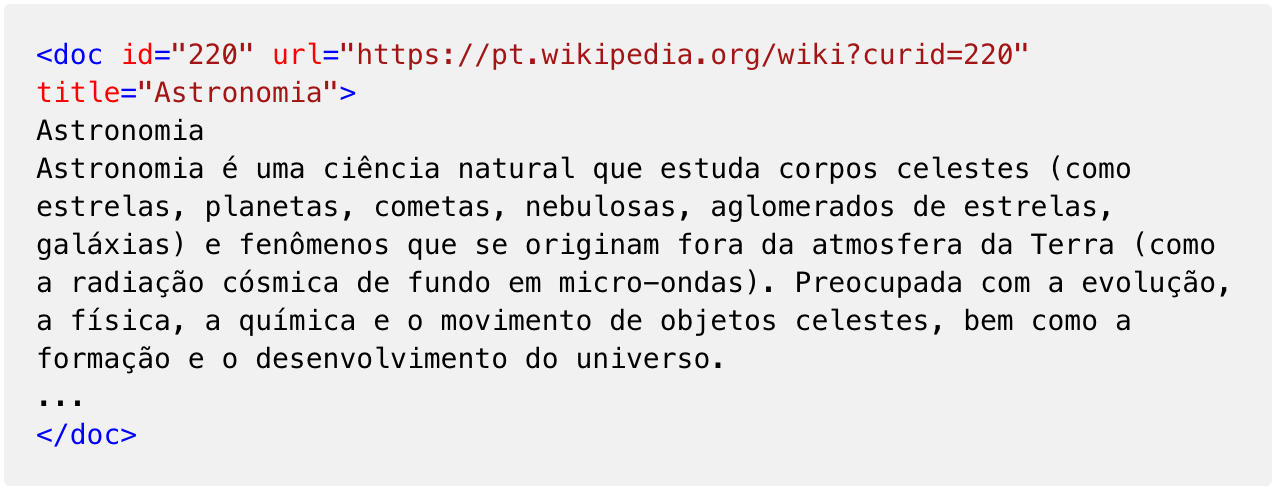
\includegraphics[width=\textwidth]{wikiextractor.png}
        \fonte{Made by the author.}
    \end{minipage}
\end{figure}

It is also possible to save this as only one text file just by changing the tool arguments.
At the time of writing, there were 1.000.400 documents in the ptwiki-dump.

\subsubsection{Custom preprocessing}

In order to cleanup the sentences for generating the Word embedding models we did some custom pre-processing\footnote{\url{https://github.com/eberlitz/pt-br-word-embeddings/blob/master/scripts/preprocess.py}} based on \citetexto{Hartmann2017} preprocessing scripts. Some changes were made to do some cleaning as follows:

\begin{itemize}
    \item Break an entire document into multiple sentences using the 
    \textbf{nltk.data.load ('tokenizers/punkt/portuguese.pickle')}. (Natural Language Toolkit - NLTK is a leading platform for building Python programs to work with human language data, and it has a sentence segmentation tool called \textbf{punkt}.)
    \item Do not change the current letter case. (Later we'll use a Syntactic parser that has better accuracy if we maintain this)
    \item Remove sentences with less than 4 tokens (as it does not add meaningful value to the corpus we can remove very short sentences).
    \item Allow abbreviations, like 'Dr.'.
    \item Keep words with '-', like 'guarda-chuva' (which means umbrella in English).
    \item All emails are mapped to EMAIL token.
    \item All numbers are mapped to 0 token.
    \item All URLs are mapped to URL token.
    \item Different quotes are standardized.
    \item Different kinds of hyphenation are standardized.
    \item HTML strings are removed.
    \item All text between brackets is removed.
\end{itemize}

With this, we ended up with the final 1.6GB PT-BR corpus file which contains 9.896.520 sentences, 251.193.592 tokens, and 3.137.040 unique tokens.

% --------------------------------------------------------

\subsection{PALAVRAS annotated corpus generation}\label{chap:methodsandmaterials:palavras}

To annotate all sentences of the corpus with syntactic tags, we used the software PALAVRAS developed by \citetexto{bick2000palavras}, which is an automatic parser for Portuguese.

First, we tried to use the parser with multiple sentence files of 1MB. However, the parser was taking too much time to execute and sometimes errors occurred. So we wrote a Python script that sends sentences in batches to the PALAVRAS parser and saves the results. Also, we have used parallel computing doing this process times the number of cores on the machine. Although, we first run this on a i5 2.4GHz computer with 4 cores, achieving an average speed of 16 sentences per second, which means that for all 9.896.520 sentences it would take 7 days to complete. We have tried other techniques attempting to increase the speed, but the bottleneck was indeed in the parser tool. 
With this problem at hand, \textit{UNISINOS Programa de Pós-graduação em Computação Aplicada} (PPGCA) granted us access to the \textit{Semantics} server (Intel(R) Xeon(R) CPU E5-2620 v4 @ 2.10GHz with 32 cores and 128GB of RAM). With 32 cores the parsing step should be concluded in 24 hours.

One more problem that we had is that the PALAVRAS could not parse some of the sentences. Since we were running the parser in batches, this means that if one sentence failed, we lost all the parsed sentences in the batch. Also, as this process would take too long, we had to implement some way to continue the process if some fatal error occurred. With this in mind, we converted the sentences file to an SQLite table with three columns (id, text and parsed text). With this whenever we start the parsing process, we can continue from where it stopped.

With this solution implemented, we created a docker image and started running in the Semantics machine. The overall process took 38 hours. 24 hours to process 8.916.000 sentences using batches of 30, and 14 hours to process the remaining ones without sending in batches. Resulting in a 15GB corpus file.

% --------------------------------------------------------

\subsection{Common Word Embeddings generation}\label{chap:methodsandmaterials:wegeneration}

In order to have a base for comparison, we generated all models that were used by \citetexto{Hartmann2017}. In this case, FastText, Wang2vec, Word2vec and GloVe using different dimensions values like 50, 100, 300, 600 and 1000 \cite{bojanowski2016enriching, Ling:2015:naacl, Mikolov2013DistributedRO, Pennington2014}. Also, the CBOW and Skip-gram were used for the models that have this option.
For this, we downloaded all those model generation tools from GitHub, compiled into a docker image, and use as input our corpus text file. We only created some script to run this several times with different dimension sizes as it took several hours to complete.

% --------------------------------------------------------

\subsection{DEPS Word Embedding generation}\label{chap:methodsandmaterials:depsgeneration}

In order to generate the DEPS (dependency-based syntactic contexts) word embedding model proposed by \citetexto{Levy2014}, we got the source code called \textit{word2vecf} from their website\footnote{\url{https://levyomer.wordpress.com/2014/04/25/dependency-based-word-embeddings/}}. The input required by this model is three files, a word, context vocabulary, and a contexts file. 
The vocabulary files are just a list of words or contexts with the total number of occurrences. The contexts file is a multiline context per word, where one word can have multiple contexts. In the form of "<\textit{word}> <\textit{dependency-relation}>\_<\textit{referred-word}>".

In order to generate this file from our corpus we got the annotated output from the PALAVRAS parser and extracted the syntactic tags. This process is shown by in ~\autoref{fig:deps-context}.

\begin{figure}[h]
    \caption{DEPS contexts generation for a single parsed sentence. Left: Sample output from the PALAVRAS parser for the sentence \textit{"A astronomia é uma das mais antigas ciências."} (Astronomy is one of the oldest sciences). Right: Sample of our generated contexts file for an annotated sentence.}
    \label{fig:deps-context}
    \centering%
    \begin{minipage}{.95\textwidth}
        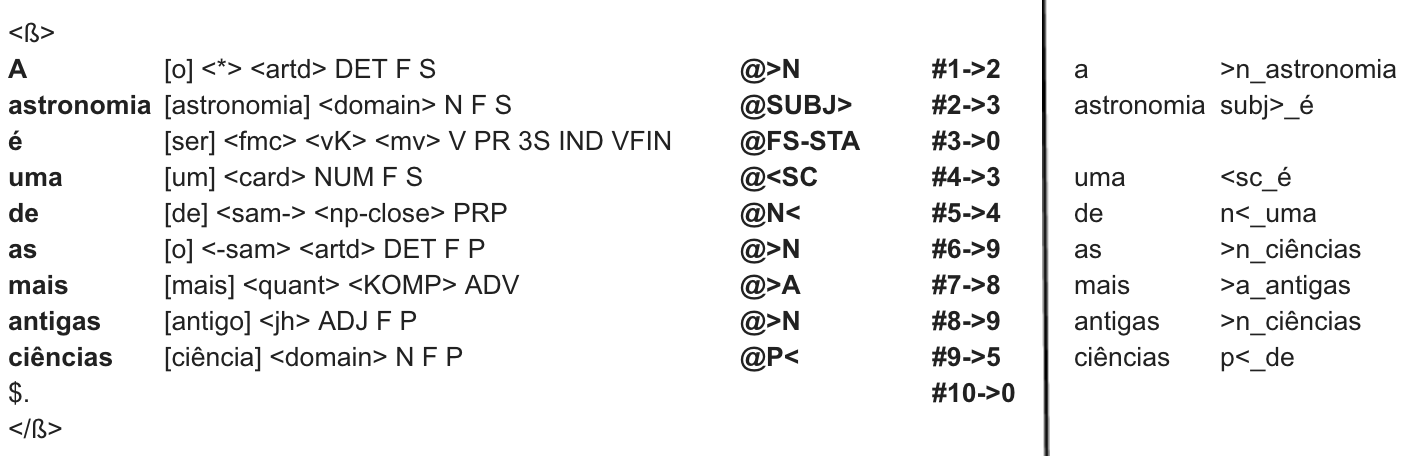
\includegraphics[width=\textwidth]{deps-context.png}
        \fonte{Made by the author.}
    \end{minipage}
\end{figure}

The generation of this three files was not trivial and the implemented code to do so had to use a map-reduce approach in order to use all computation resources available. It took 14 hours to process all 9.896.000 parsed sentences with an average speed of 196,2 sentences per second.
After we had the input files, we just run the \textit{word2vecf} tool which took some hours to complete. We generated models with different dimensions values as 50, 100, 300, 600 and 1000.